\documentclass{article}

\usepackage{graphicx}
\usepackage{changepage}
\usepackage{booktabs}

\begin{document}

\section{Diagramma ER}

\begin{adjustwidth}{-50cm}{-50cm}
    \vspace{\fill}
    \begin{center}
        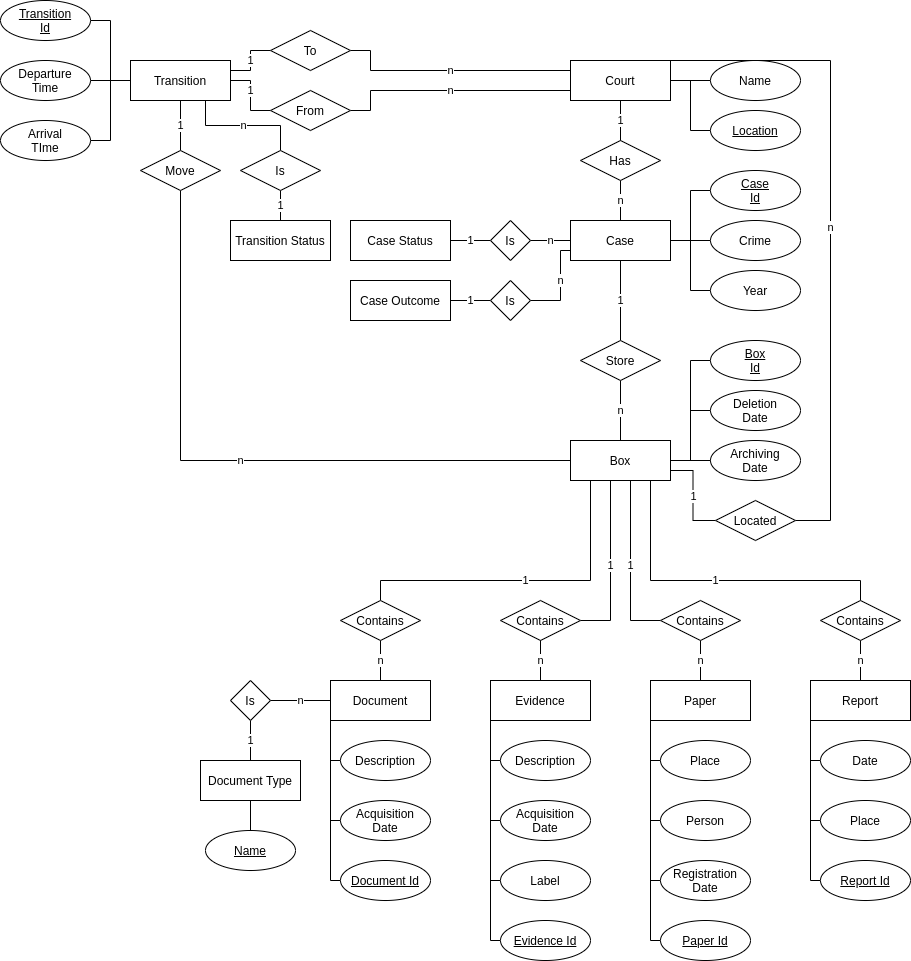
\includegraphics[scale=0.50]{../images/er.png}
    \end{center}
    \vspace{\fill}
\end{adjustwidth}

\newpage
\section{Ipotesi}

\begin{itemize}
    \item Non possono essere eliminati elementi singoli all'interno di una scatola, ma è necessario eliminare la scatola intera.
\end{itemize}

\section{Mapping}

Court(\underline{Location}, name) \\
Case(\underline{CaseId}, \textit{Court}, \textit{Status}, \textit{Outcome}, Crime, Year) \\
CaseStatus(\underline{Name}, Description) \\
CaseOutcome(\underline{Name}, Description) \\
Box(\underline{BoxId}, \textit{Case}, \textit{Location}, ArchivingDate, DeletionDate)

\noindent \\
Evidence(\underline{EvidenceId}, \textit{Box}, Description, AcquisitionDate, Label) \\
Paper(\underline{PaperId}, \textit{Box}, Place, Person, RegistrationDate) \\
Report(\underline{ReportId}, \textit{Box}, Place, Date) \\
Document(\underline{DocumentId}, \textit{Box}, \textit{Type}, Description, AcquisitionDate) \\
DocumentType({\underline{Name})

\noindent \\
Transition(\underline{TransitionId}, \textit{Box}, \textit{From}, \textit{To}, \textit{Status}, DepartureTime, ArrivalTime) \\
TransitionStatus(\underline{Name}, Description)

\section{Normalizzazione}

\subsection{Prima forma normale}
Per rendere tutti i campi atomici sono necessarie le seguenti modifiche:
\begin{enumerate}
    \item Box.ArchivingTime $\rightarrow$ ArchivingDate, ArchivingTime
    \item Paper.Person $\rightarrow$ CF, Name, Surname
\end{enumerate}

\noindent
Aggiungendo dunque la tabella ``Person(\underline{CF}, Name, Surname)" e modificando la tabella Paper in  ``Paper(\underline{PaperId}, \textit{Box}, Place, \textit{Person}, RegistrationDate)''

\subsection{Seconda forma normale}

Tutte le tabelle sono in seconda forma normale, in quanto non esistono campi non chiave
che dipendono da una porzione di una chiave candidata.

\subsection{Terza forma normale}

Tutte le tabelle sono in terza forma normale, in quanto non esistono campi non chiave
che dipendono da campi non chiave

\subsection{Forma normale di Boyce-Codd}

Tutte le tabelle sono nella forma normale di Boyce-Codd, in quanto tutti i
campi determinanti sono superchiavi.

\section{Tabelle enumerabili}

\subsection{Transition status}
\begin{table}[h]
    \begin{center}
        \begin{tabular}{c|l}
            \toprule
            \textbf{Value} &
            \textbf{Description}                                           \\
            \midrule
            Requested      & The destintion court requested the transition \\
            Accepted       & The origin court accepted the transition      \\
            Transiting     & The transition is taking place                \\
            Completed      & The transition is completed                   \\
            \bottomrule
        \end{tabular}
    \end{center}
\end{table}

\subsection{Case status}
\begin{table}[h]
    \begin{center}
        \begin{tabular}{c|l}
            \toprule
            \textbf{Value} &
            \textbf{Description} \\
            \midrule
            Preliminary    &     \\
            First          &     \\
            Second         &     \\
            Canceled       &     \\
            Prescribed     &     \\
            \bottomrule
        \end{tabular}
    \end{center}
\end{table}

\subsection{Case outcome}
\begin{table}[h]
    \begin{center}
        \begin{tabular}{c|l}
            \toprule
            \textbf{Value} &
            \textbf{Description} \\
            \midrule
            Condemned      &     \\
            Acquitted      &     \\
            \bottomrule
        \end{tabular}
    \end{center}
\end{table}

\end{document}
